% ------------------------------------------------------------------------------
% TYPO3 CMS 8.5 - What's New - Chapter "Backend User Interface" (German Version)
%
% @author	Michael Schams <schams.net>
% @license	Creative Commons BY-NC-SA 3.0
% @link		http://typo3.org/download/release-notes/whats-new/
% @language	English
% ------------------------------------------------------------------------------
% LTXE-CHAPTER-UID:		07b25346-95b1df21-a6ebe09a-49f53f41
% LTXE-CHAPTER-NAME:	Backend User Interface
% ------------------------------------------------------------------------------

\section{Backend User Interface}
\begin{frame}[fragile]
	\frametitle{Backend User Interface}

	\begin{center}\huge{Kapitel 1:}\end{center}
	\begin{center}\huge{\color{typo3darkgrey}\textbf{Backend User Interface}}\end{center}

\end{frame}

% ------------------------------------------------------------------------------
% LTXE-SLIDE-START
% LTXE-SLIDE-UID:		e4beee9d-131606d6-ca1ca631-c27d1262
% LTXE-SLIDE-ORIGIN:	e00709d6-ccb8a4d0-1cca1d28-431a00a5 English
% LTXE-SLIDE-TITLE:		#77910: New Form Framework (1)
% ------------------------------------------------------------------------------
\begin{frame}[fragile]
	\frametitle{Backend User Interface}
	\framesubtitle{Neues Form Framework (1)}

	\begin{itemize}
		\item In TYPO3 CMS 8.5 wurde ein neues, flexibles Framework integriert um Formulare zu erstellen
		\item Dieses ersetzt den auf ExtJS basierenden \textit{Form Wizard}
		\item Der neue \textit{Form Editor} verwendet jQuery und  eine moderne Architektur um eine hohe Flexibilität und Erweiterbarkeit zu gewärleisten
		\item Das Framework ist hoch flexibel; die Konfiguration wird über YAML-Dateien durchgeführt
		\item Die Feature-Liste ist beindruckend\newline
			\small(ein komplette Dokumentation wird in Kürze verfügbar sein)\normalsize
		\item Ein Demonstrationsvideo ist auf YouTube verfügbar:\newline
			\url{https://www.youtube.com/watch?v=F9sTAOEcTI0}
	\end{itemize}

\end{frame}
% ------------------------------------------------------------------------------
% LTXE-SLIDE-START
% LTXE-SLIDE-UID:		1e167370-96c1432d-79ede1c1-bc9ff2ba
% LTXE-SLIDE-ORIGIN:	3bbca669-629eab1c-0230fd06-71e7071c English
% LTXE-SLIDE-TITLE:		#77910: New Form Framework (2)
% ------------------------------------------------------------------------------
\begin{frame}[fragile]
	\frametitle{Backend User Interface}
	\framesubtitle{Neues Form Framework (2)}

	\begin{figure}
		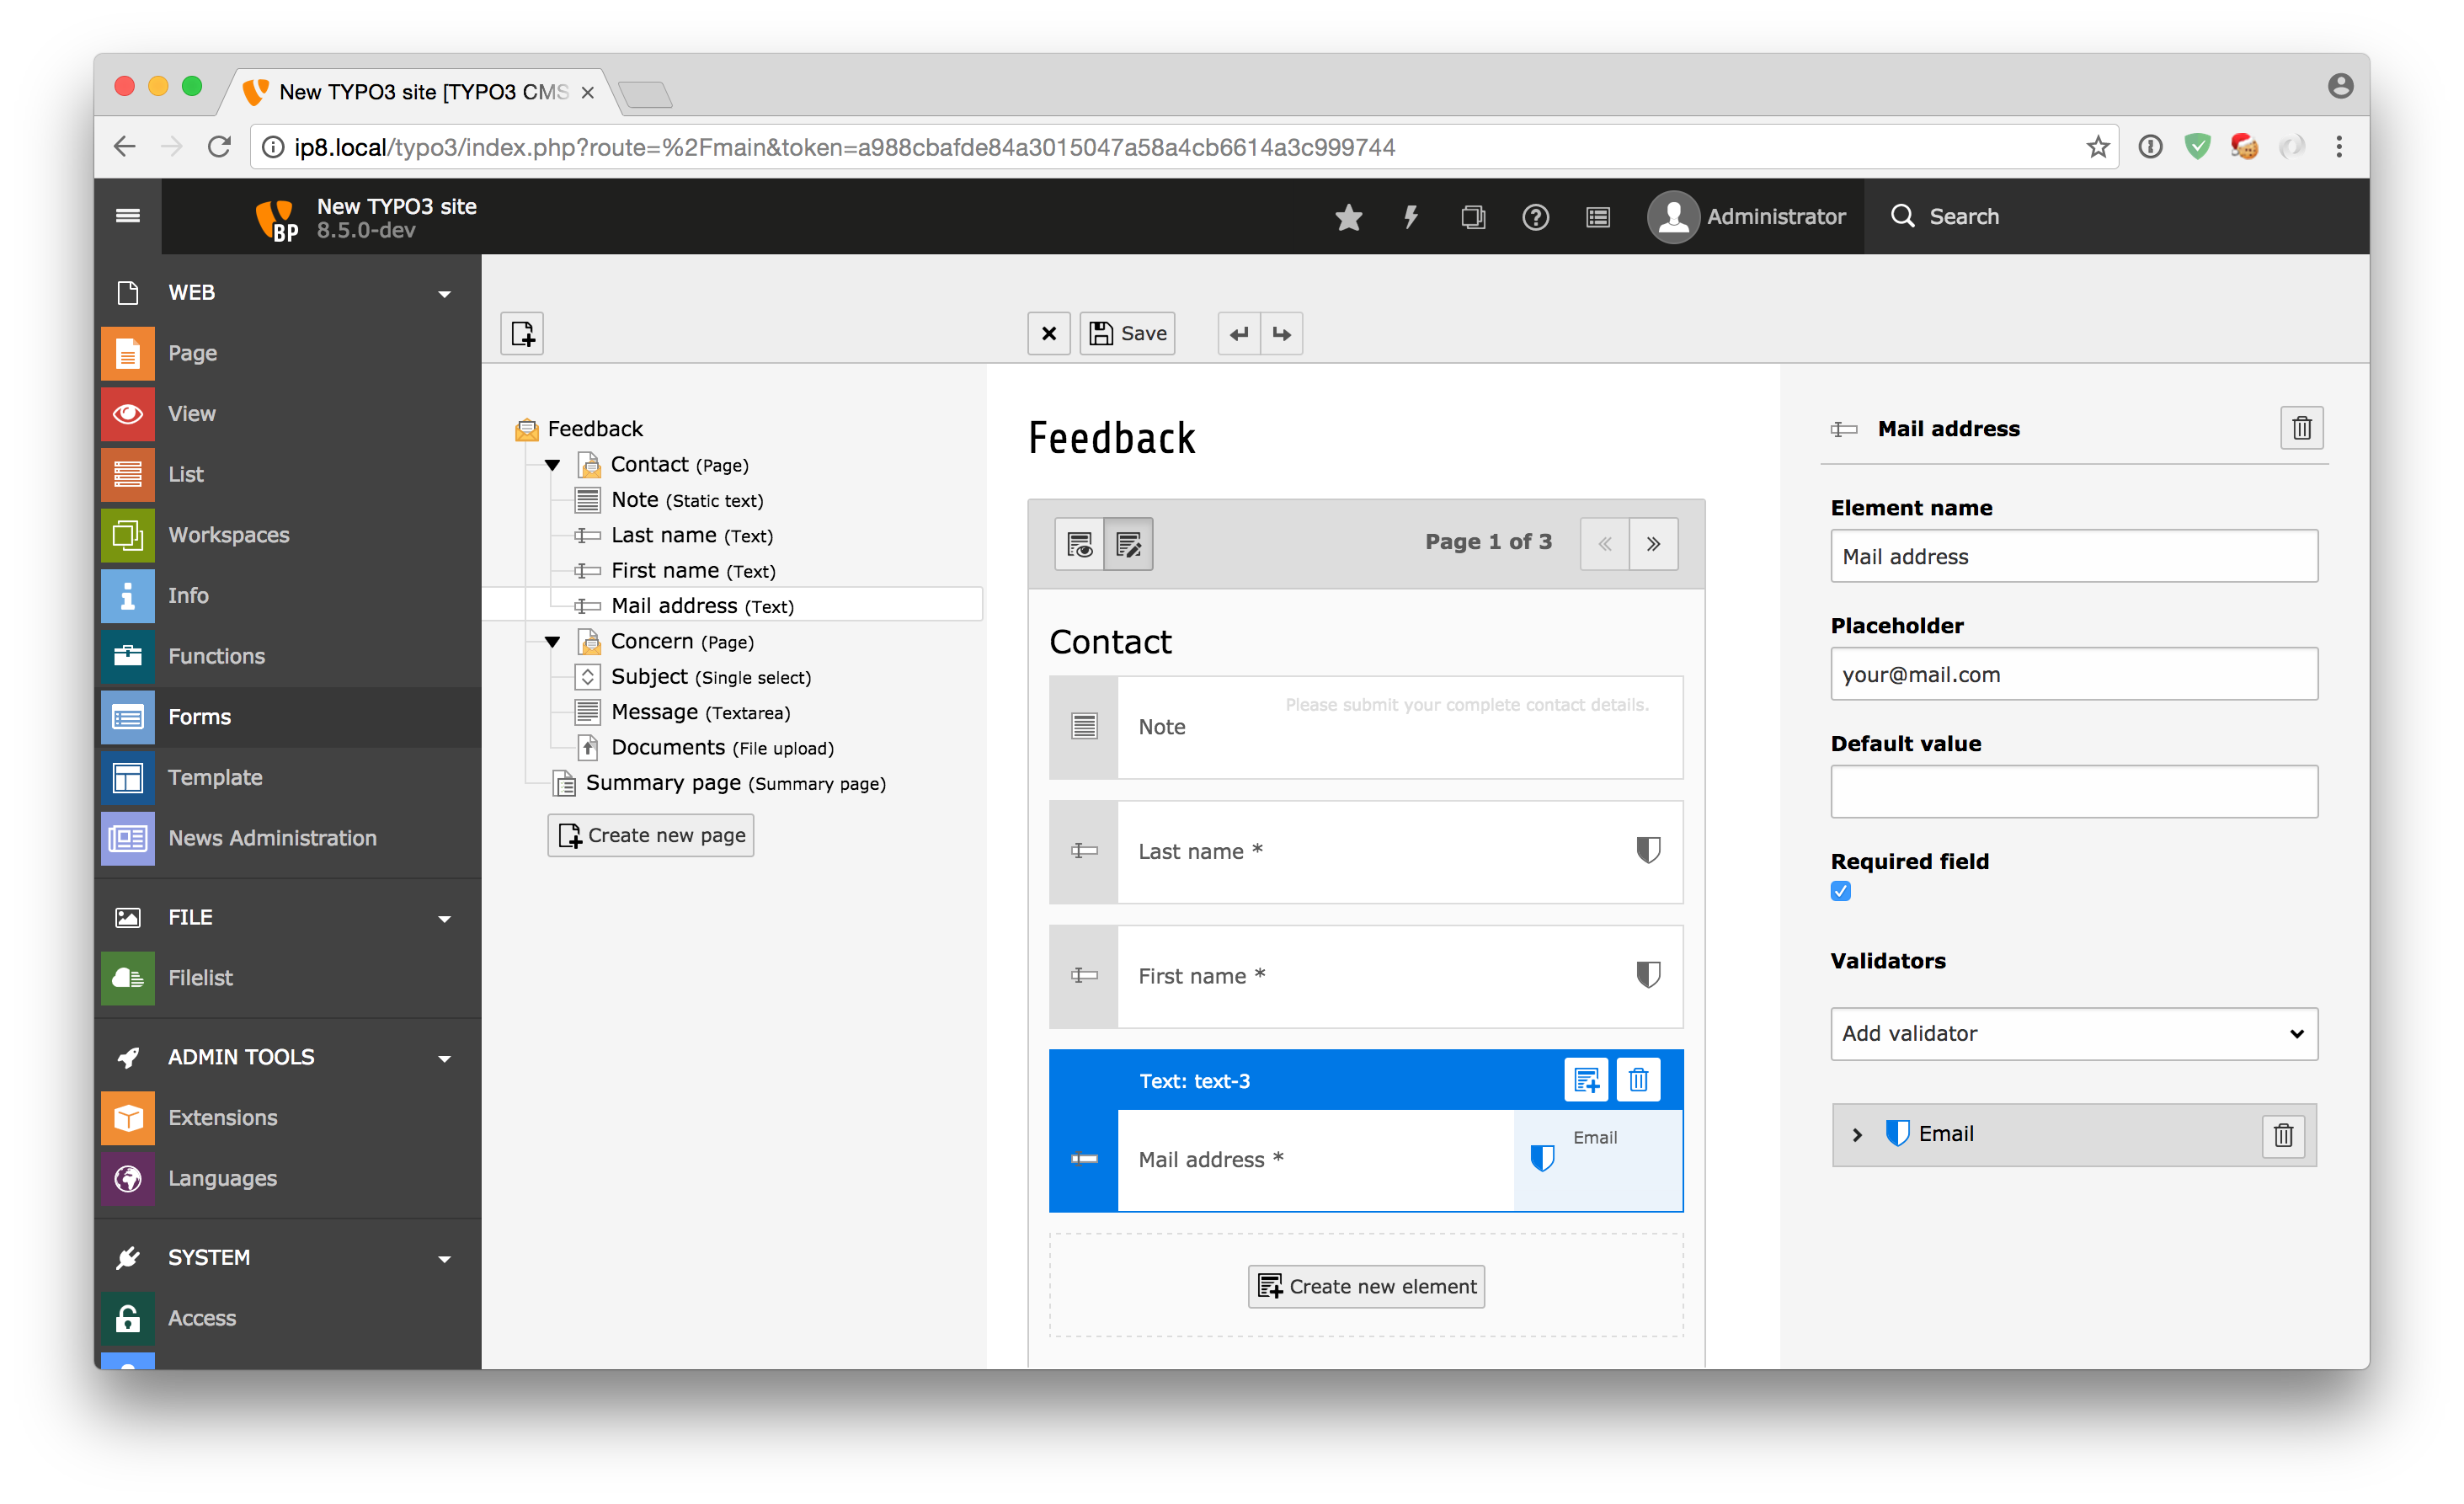
\includegraphics[width=0.8\linewidth]{BackendUserInterface/form-framework-1.png}
	\end{figure}

\end{frame}

% ------------------------------------------------------------------------------
% LTXE-SLIDE-START
% LTXE-SLIDE-UID:		b403e9dc-8f28e6ec-b2fe1afd-0aacc507
% LTXE-SLIDE-ORIGIN:	b91ec75b-7aa7b566-b523ca5f-f9ba3cde English
% LTXE-SLIDE-TITLE:		#77910: New Form Framework (3)
% ------------------------------------------------------------------------------
\begin{frame}[fragile]
	\frametitle{Backend User Interface}
	\framesubtitle{Neues Form Framework (3)}

	\begin{figure}
		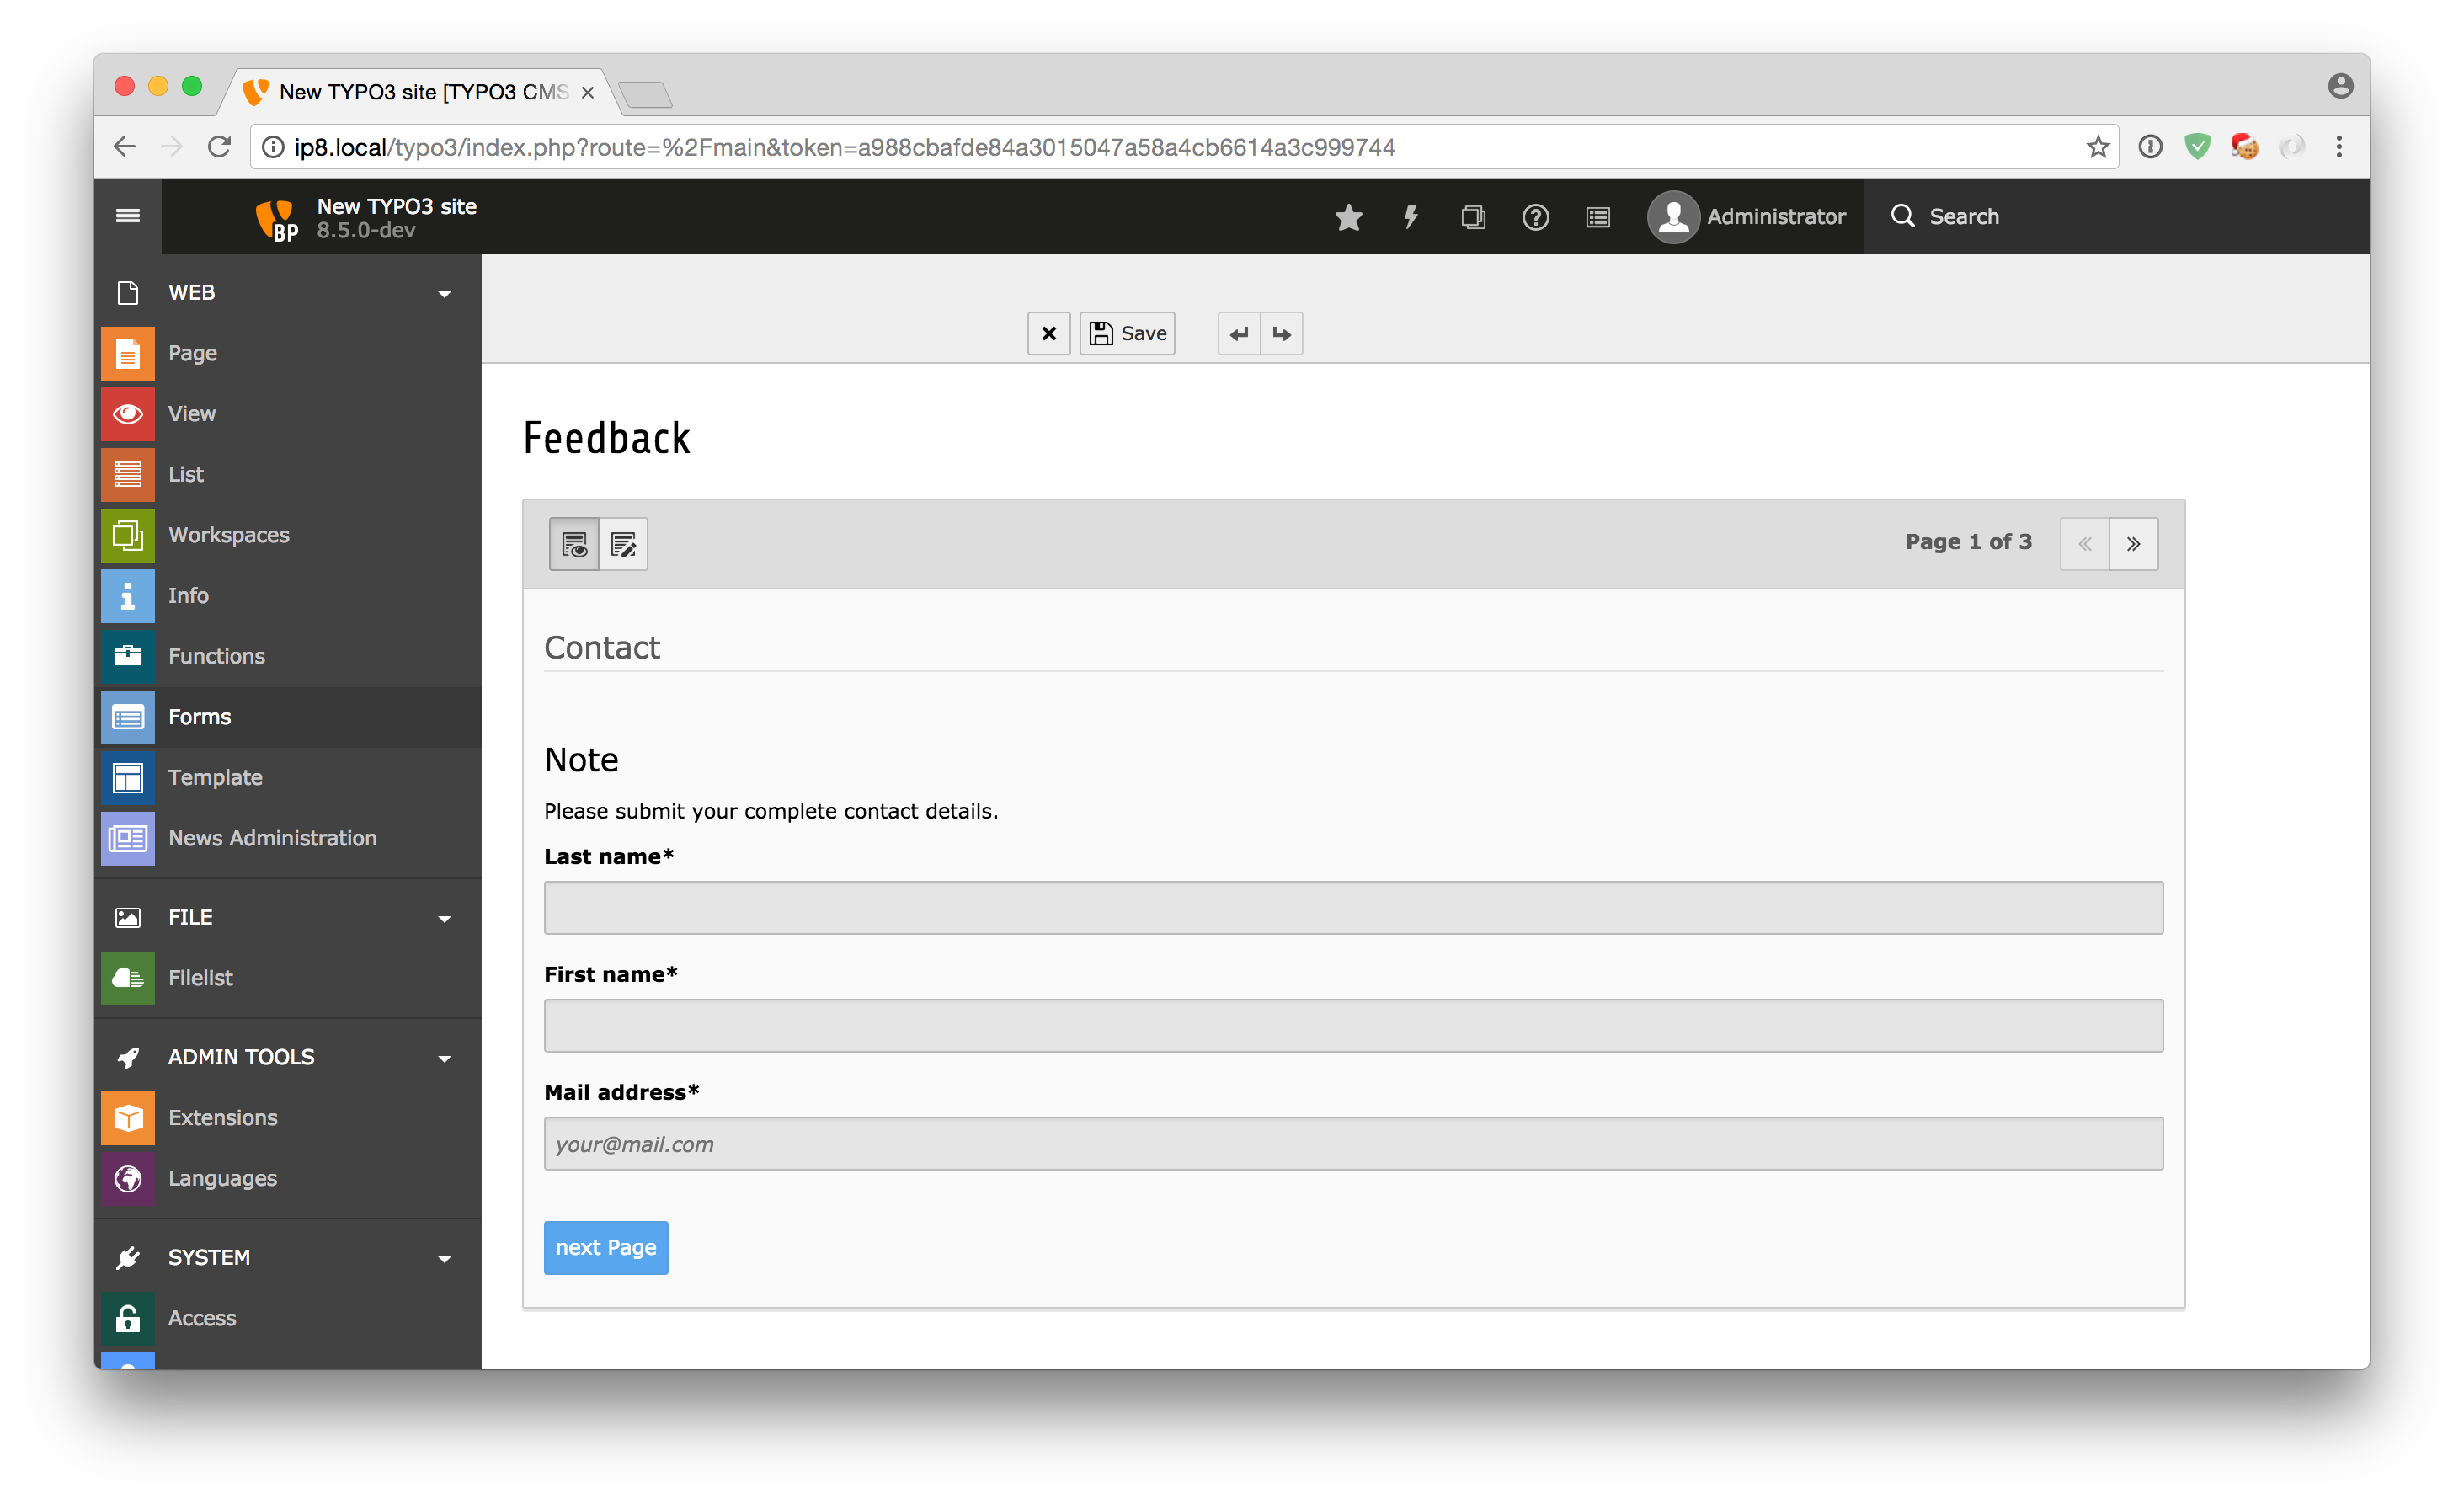
\includegraphics[width=0.8\linewidth]{BackendUserInterface/form-framework-2.png}
	\end{figure}

\end{frame}


% ------------------------------------------------------------------------------
% LTXE-SLIDE-START
% LTXE-SLIDE-UID:		1539736d-c0bd7207-b92524a9-4069e4e1
% LTXE-SLIDE-ORIGIN:	c41b2f21-fb92bb80-56e7ddc9-1c725e34 English
% LTXE-SLIDE-TITLE:		CKEditor Integration
% ------------------------------------------------------------------------------
\begin{frame}[fragile]
	\frametitle{Backend User Interface}
	\framesubtitle{CKEditor Integration}

	\begin{columns}[T]
		\begin{column}{.5\textwidth}
			In das TYPO3 CMS Backend wurde die nächste Generation des Rich-Text-Editing implementiert:
			\textbf{CKEditor}.\newline
			Der aktuelle Status ist explizit als \textit{experimental} gekennzeichnet - daher wird
			die Extension per Default nicht installiert.\newline
			Weitere Informationen des Open Source Editors finden sich hier: \url{http://ckeditor.com}
		\end{column}
		\begin{column}{.5\textwidth}
			\begin{figure}\vspace*{-0.4cm}
				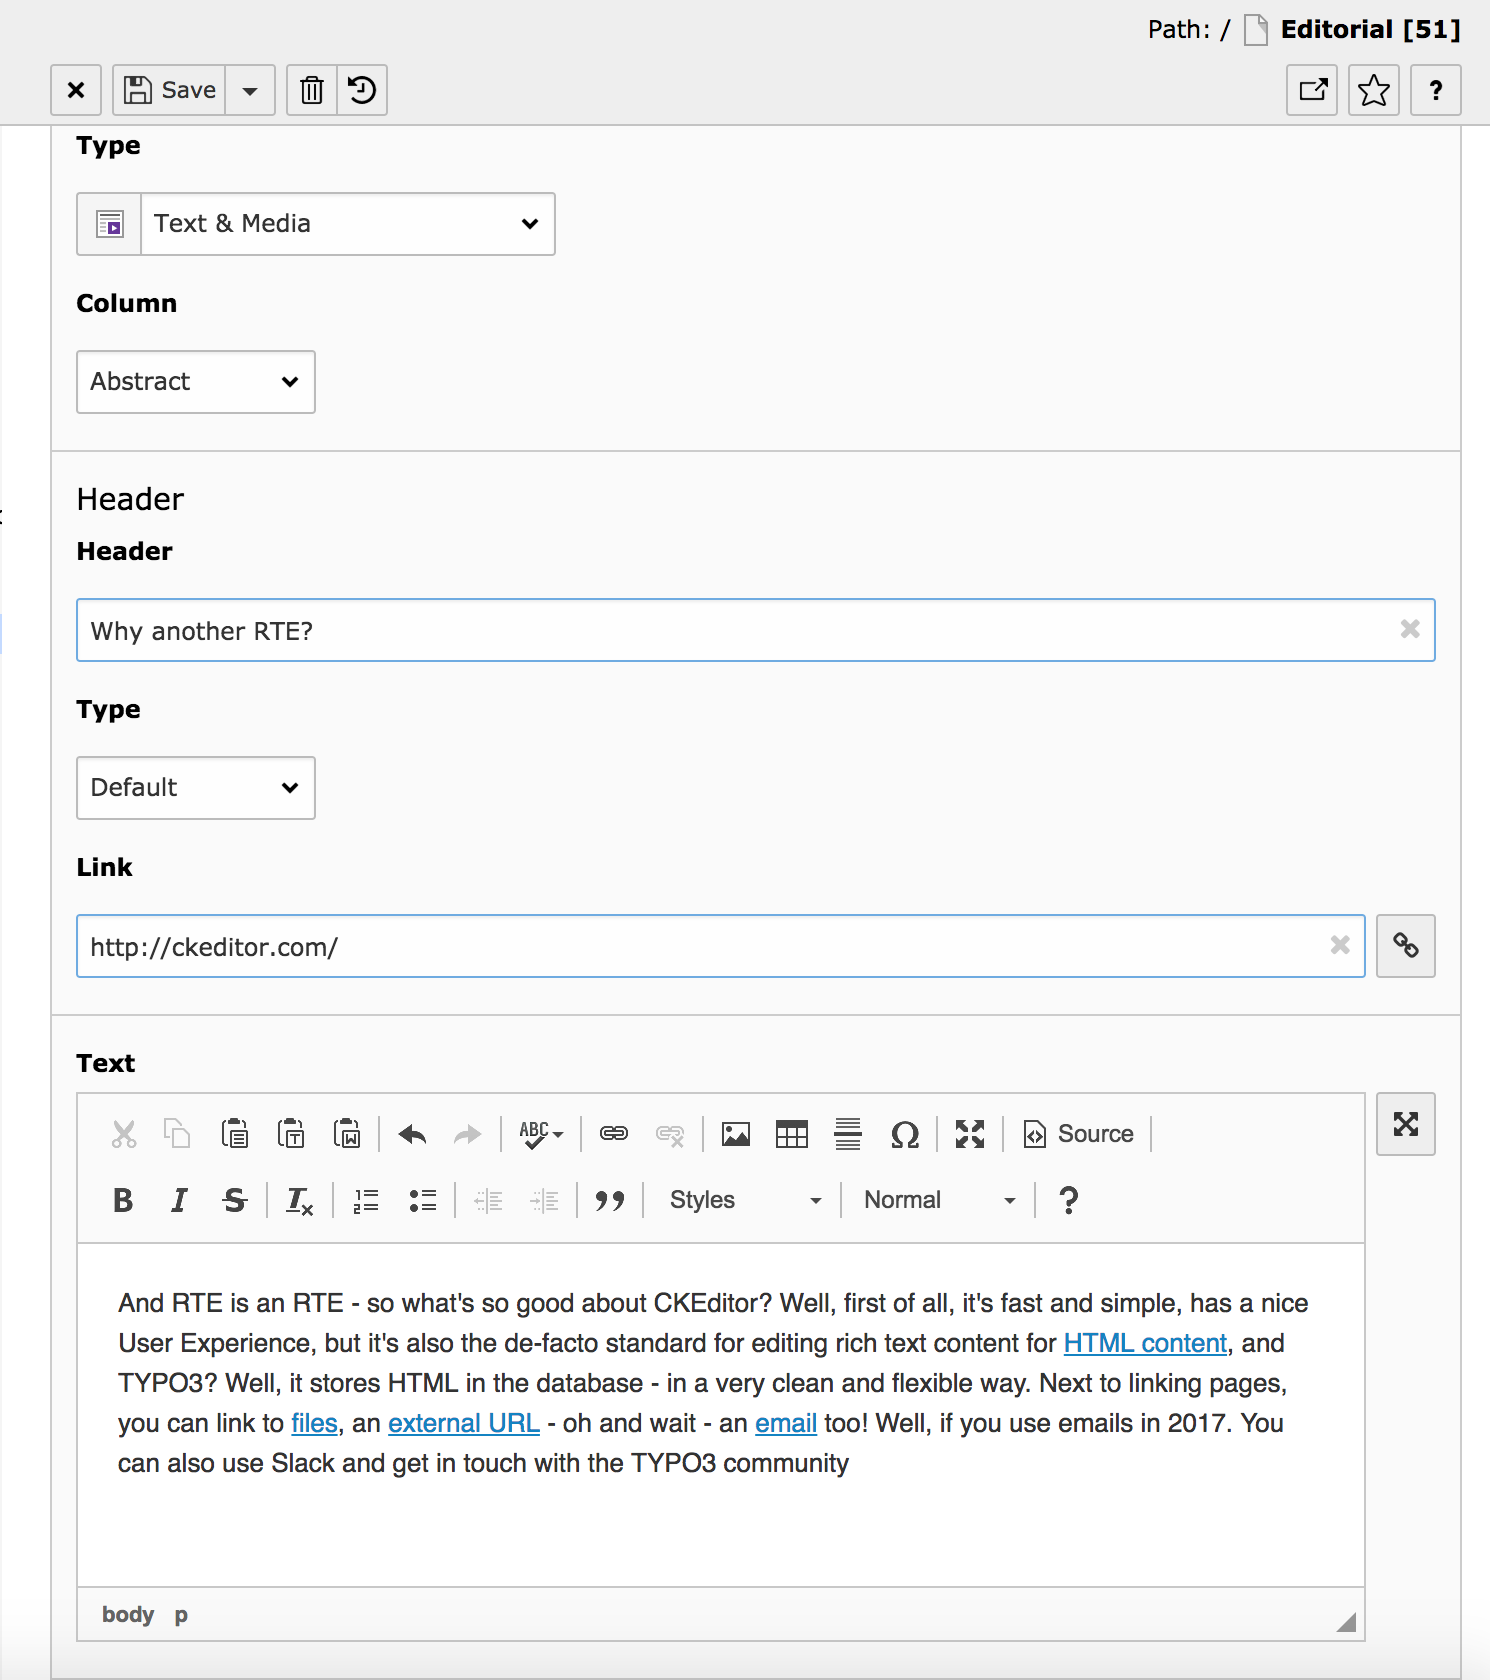
\includegraphics[width=0.8\linewidth]{BackendUserInterface/ckeditor.png}
			\end{figure}
		\end{column}
	\end{columns}

\end{frame}



% ------------------------------------------------------------------------------
% LTXE-SLIDE-START
% LTXE-SLIDE-UID:		feb133ac-f932d727-dd8e0e86-5355e020
% LTXE-SLIDE-ORIGIN:	c9dc360d-cf218f95-03f53731-03d821ad English
% LTXE-SLIDE-TITLE:		#78383: Field positions in tabs streamlined (TCA)
% ------------------------------------------------------------------------------
\begin{frame}[fragile]
	\frametitle{Backend User Interface}
	\framesubtitle{Position and Anordnung von Elementen}

	\begin{itemize}
		\item Die Anordnung und Position zahlreicher Felder im Backend wurde neu gestaltet
		\item Das Ziel war es, die Erwartungen der User besser zu abzubilden, wenn es darum geht, wo bestimmte Felder zu finden sind
		\item Das ist inbesondere für wiederkehrende Felder und generische Kategorien von zahlreichen Datensätzen wichtig
		\item Extension-Authoren sind angehalten den Richtlinien hinsichtlich der spezifischen Positionen und Anordnungen zu folgen \href{https://docs.typo3.org}{official documentation}

			% TODO: update link above (waiting for Doc and Core Team to finish documentation)

	\end{itemize}

	\begin{itemize}
		\item \textit{Backend consistency is king!} :-)
	\end{itemize}

\end{frame}

% ------------------------------------------------------------------------------
